\documentclass[12pt, a4paper]{article}
\usepackage[margin=2.0cm]{geometry}
\usepackage{stmaryrd}
\usepackage{amsmath}
\usepackage{amssymb}
\usepackage{enumerate}
\usepackage{bbold}
\usepackage{dsfont}
\usepackage{algorithm2e}
\usepackage{changepage}
\usepackage{undertilde}
\usepackage{hyperref}
\hypersetup{pdftex,colorlinks=true,allcolors=blue}
\usepackage{hypcap}
\usepackage{fancyhdr}
\usepackage{float}
\usepackage[english]{babel}
\usepackage{graphicx}
\usepackage{caption}
\usepackage{subcaption}
\usepackage{wrapfig}
\usepackage{multicol}

\pagestyle{fancy}
\fancyhf{}
\lhead{dc14770}
\rhead{HPC CW2}

\setlength{\parskip}{.1in}
\setlength{\parindent}{0in}
\setlength{\columnsep}{0.5cm}

\begin{document}

  \vspace{.1in}
	\begin{center}
	{ \Large High Performance Computing }

  \end{center}
  \begin{center}

	Dylan Cope, Coursework 2 Report

	\vspace{.1in}

	\end{center}

  \section*{Introduction}

  \begin{multicols}{2}

    Starting with the serial optimisations performed in the first coursework, this report outlines the optimisations made using OpenCL to parallelise the program. For this coursework the Lattice-Boltzmann algorithm was run on four 2D grids of sizes 128x128, 128x256, 256x256 and 1024x1024 to analyse how the optimisations are effected by scaling. Figure \ref{serial} is the runtimes for each input with the starting codebase. These runtimes will be used as the baseline to assess future optimisations.

    \begin{figure}[H]
      \caption{} \vspace{-0.8cm}
      \label{serial}
      \begin{center}
        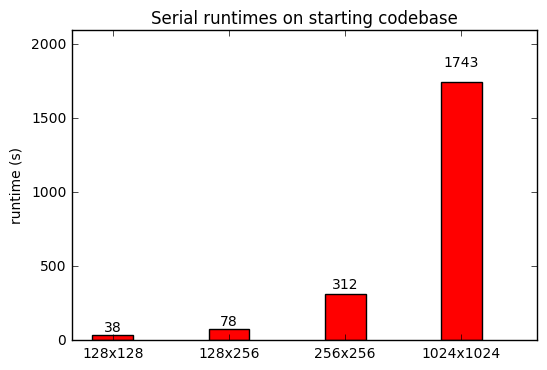
\includegraphics[width=0.4\textwidth]{figures/serial}
      \end{center}
    \end{figure}

  \end{multicols}

  \section*{Basic OpenCL Kernels}

  \begin{multicols}{2}

    \begin{figure}[H]
      \caption{} \vspace{-0.8cm}
      \label{wgs}
      \begin{center}
        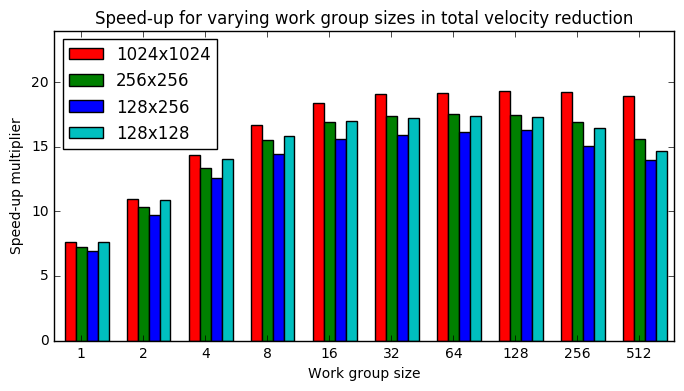
\includegraphics[width=0.4\textwidth]{figures/workgroupsize}
      \end{center}
    \end{figure}

  \end{multicols}

\end{document}
